\section{UML}
\label{sc:UMLB}
UML ist die meiste benutzte und beliebte Modellierungssprache, deswegen sie ist heute eine der dominierenden Sprachen für die Modellierung von betrieblichen Anwendungs- bzw. Softwaresystemen. Der erste Kontakt zu UML besteht häufig darin, dass UML-Diagramme im Rahmen von Softwareprojekten zu erstellen, zu verstehen oder zu beurteilen sind. UML-Diagramme gelten als Standard bei objektorientierter Modellierung\cite{MT005}.
\subsection{Eignung}

Aus meine eigene Erfahrung und meiner persönlichen Sicht sind die starke punkte des Einsatzs von UML in der breiten Unterstützung sämtlicher objektorientierter Grundsätze. 
Man kann an vielen Stellen ein und dasselbe Problem auf unterschiedliche Art und Weise lösen, ohne sich dabei durch die Vorgaben der Sprache eingeengt zu fühlen. Diese Sprach ermöglicht an den Anwender, einfach nach eigenen Ideen und Vorstellungen zu modellieren.\\
Besonders Vorteilhaft erscheint die Tatsache, dass UML auch die Erweiterungsmöglichkeiten durch eigene Sprachkonstrukte vorsieht (Metamodell), und damit wirklich jedem das Recht anbietet, den eigenen Notationsrahmen zu erschaffen. Diese Möglichkeit sollte aber nur in äußersten Notfällen (wenn es nicht anders geht) verwendet werden, da man sonst der Gefahr, sich vom Standard zu entfernen, entgegenläuft \cite{MT015}.
Die UML hat eine starke Affinität zu den objektorientierten Programmiersprachen C++  und Java. Zusätzlich wurde die UML deutlich um weitere Diagrammtypen ergänzt die speziell für den Entwurf von Software-Architekturen konzipiert sind.
Der UML-Standard bietet mit insgesamt vierzehn jeweils spezialisierten Darstellungen professionelle Unterstützung für unterschiedlichste Anwendungsfälle. Die Diagrammformen lassen sich unterteilen in Darstellungsformen zur Modellierung von Strukturen und zur Modellierung von Verhalten klassifizieren.

Andere sehr wichtiger Vorteil von UML,dass sie in viele verschiedenen Bereichen benutzbar ist. Obwohl UML ursprünglich für die Modellierung von Software-Systemen entwickelt worden ist, aber sie ist nicht eingeschränkt und sie ist auch für Organisationsprojekte einsetzbar. Durch die Möglichkeit, Prozesse visualisieren zu können, ist es im Anschluss möglich, diese zu analysieren und zu verbessern.

Die Verwendung von UML als "gemeinsame Sprache" führt zu einer Verbesserung der Zusammen¬arbeit zwischen Technikern und Nicht-Technikern, darunter fallen Projektleiter, Business Analysten, Softwarearchitekten, -designer und  entwickler. Sie hilft, Systeme besser zu verstehen, Möglichkeiten der Vereinfachung und/oder Wiederverwendbarkeit aufzudecken und mögliche Risiken besser zu erkennen. Durch frühzeitige Erkennung von Fehlern in der Analyse- bzw. Designphase eines Projekts können die Kosten während der Implementierungsphase verringert werden. Die Möglichkeit des Round¬trip Engineerings bietet vor allem für Entwickler eine enorme Zeitersparnis.\\


Weiterer Vorteil liegt in der Standardisierung der UML. Die  UML bietet eine fast perfekte Grundlage für die Kommunikation der verschiedenen Entwicklungsteams miteinander. Diagramme können nun nicht nur von den Fachleuten der Software –Firma , sondern auch von den außerhalb stehenden verstanden und verbessert werden. Lästiges  Einarbeiten in die verschiedenen Notationen entfällt, falls sich alle grundsätzlich an die UML halten. 
Weiterer Vorteil liegt in der zunehmenden Verbreitung der Unified Modeling Language. Die exakten Zahlen sind zwar noch schwer abzuschätzen, es zeichnet sich jedoch ein wachsender Trend für den Einsatz der UML ab\cite{MT015}.\\
Man kann die Vorteile von UML in vier wichtigste Punkte zusammenfassen wie folge:\\

- Die Vereinheitlichung der Terminologie und die Standardisierung der Notation
führen zu einer massiven Erleichterung der Verständigung zwischen allen
Beteiligten\cite{MT016}.\\
- Die UML wächst mit Ihren Anforderungen an die Modellierung. Sie können mit der
Erstellung einfacher Modelle beginnen, aber auch sehr komplexe Sachverhalte im
Detail modellieren, da die UML eine mächtige Modellierungssprache ist\cite{MT016}.\\
- Die UML baut auf bewährten und weit verbreiteten Ansätzen auf. Die UML wurde
nicht im Elfenbeinturm erstellt, sondern hat sich zu großen Teilen aus der Praxis
und aus bestehenden Modellierungssprachen heraus entwickelt. Das gewährleistet
die Einsatzfähigkeit und Praxisnähe der UML.\\
- Sie ist in viele verschiedene Bereichen einsetzbar.\\
- Experten können Ihnen mit Hilfe eines Klassendiagramms wesentlich schneller eine professionelle Analyse für ein System liefern.\\
- Weniger erforderliche Regeln innerhalb von Aktionen bedeuten weniger Programmcode und helfen dabei ein Programmdesign zu optimieren.\\
- Die Wichtigkeit von dokumentierten Anforderungen immer wieder unterschätzt. Wenn Anforderungen mit Projektstart fortlaufend schriftlich dokumentiert sind, werden Projektrisiken maßgeblich reduziert und die die Qualität von Softwareanwendungen steigt nachweislich.

\subsection{Uneignung}
UML ist eine tolle Sprache zum modellieren ein Modell von einem Program oder Software, aber es gibt eine wachsende Gemeinschaft, die Punkte einige Nachteile für einige fehlende features. Trotz des vielen Vorteilen stehen auch Nachteile gegenüber.

Die UML wird hinsichtlich semantischer Inkonsistenzen, Konstruktmehrdeutigkeiten, inadäquate Notationen und kognitiven Unzugänglichkeiten kritisiert. Dazu  verursacht die hohe Komplexität der Sprache (beispielsweise umfasst die Sprachspezifikation aktuell rund 800 Seiten)  Schwierigkeiten bei ihrer Benutzung.
Andere Nachteil sind die Werkzeuge, bisher sind keine Werkzeuge verfügbar, die den Sprachstandard vollständig unterstützen.
Die Pflege des Standards ist auch schwerfällig und leicht fehleranfällig.






Die Nachteile lassen sich nun wiederum aus dem Umfang der Sprache ableiten. UML ist sehr vielfältig, so dass auch am Anfang  sehr viel Aufwand für das Aneignen und Verstehen sämtlicher Sprachkonstrukte aufgebracht werden muss.\\ Außerdem wird man in der  Regel feststellen, dass viele Elemente sehr selten zum Einsatz kommen und damit eher als Ballast der Sprache angesehen werden\cite{MT015}.\\

Speziell für die Entwicklung der Software für eingebettete Systeme lässt sich anmerken, dass UML eine objektorientierte Modellierungssprache ist. Sämtliche Konzepte von UML können nur dann ausgenutzt werden, wenn wirklich objektorientiert programmiert wird. Es macht wenig Sinn, objektorientiert zu modellieren , wenn  anschließend kein objektorientierter Code verwendet wird. Steht kein objektorientierter Compiler zur Verfügung, sollte man sich über den Einsatz anderer Werkzeuge und Spezifikationssprachen Gedanken machen. Man kann zwar im begrenzten Maße sämtliche objektorientierte Ansätze in den „strukturierten“ Code konvertieren (also z.B. von C++ nach C überführen), das Ergebnis lässt jedoch zu wünschen übrig, insbesondere leidet die Code- Qualität / Lesbarkeit darunter\cite{MT015}.\\

Man kann die Nachteile von UML in vier wichtigste Punkte zusammenfassen wie folge:\\
- Die neue Notation muss zuerst erlernt werden. Es fallen somit Schulungskosten an
und die Mitarbeiter müssen dafür Zeit aufwenden können\cite{MT016}.\\
- Im Bereich der Software-Unterstützung ist noch einiges zu tun, bis wirklich
benutzerfreundlich mit UML gearbeitet werden kann\cite{MT016}.\\
- Durch die Vereinheitlichung der Modellierungssprachen geht die Vielfalt und
Kreativität verloren. Kleine, vielleicht gute Modelle gehen verloren\cite{MT016}.\\
- Der Wettbewerb wird durch die Monopolisierung zerstört\cite{MT016}.\\
- Sie hat viele Diagrammarten, damit die Entscheidung in der Auswahl des Diagramms schwerig ist.\\
- Für einige Modellierungsaufgaben nicht ideal geeignet, da spezifische Ausdrucksweisen fehlen.
\subsection{Fazit}

Wir versuchen in diesem Abschnitt die Eignungen und Uneignungen von UML zusammenfassen und einen Überblick darüber geben.


		
		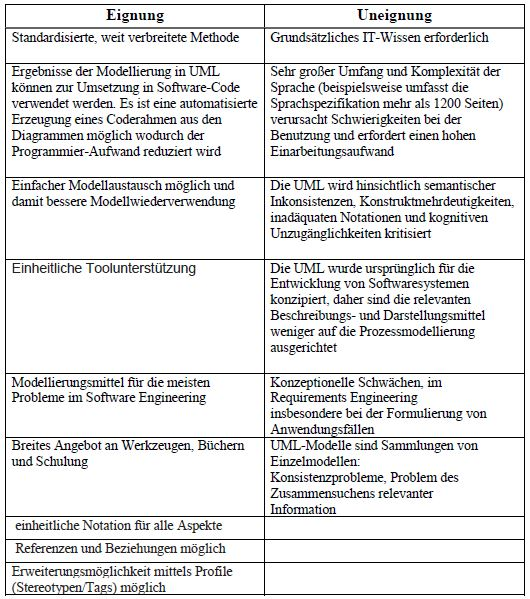
\includegraphics[scale=1]{Graphics/vornachteil.jpg} 
		\captionof{figure}{Eignung und Uneignung von UML}
		
		
		
